\section*{Тестирование и результаты}

В рамках работы был проведён анализ производительности алгоритма LZ77 на входных данных различной длины. Результаты измерений времени выполнения представлены в таблице ниже:

\begin{table}
\centering
\begin{tabular}{|c|c|c|}
\hline
\textbf{Длина строки} & \textbf{Время кодирования (с)} & \textbf{Время декодирования (с)} \\ \hline
100                  & 0.000339                       & 0.000016                         \\ \hline
1,000                & 0.025167                       & 0.000169                         \\ \hline
10,000               & 2.045418                       & 0.001115                         \\ \hline
50,000               & 43.782558                      & 0.005081                         \\ \hline
100,000              & 167.442517                     & 0.009726                         \\ \hline
200,000              & 639.585825                     & 0.021188                         \\ \hline
500,000              & 3752.310975                    & 0.060066                         \\ \hline
\end{tabular}
\caption{Результаты тестирования производительности алгоритма LZ77}
\label{tab:results}
\end{table}

\noindent Как видно из таблицы, время кодирования растёт значительно быстрее, чем время декодирования. Это объясняется тем, что процесс кодирования включает поиск совпадений в уже просмотренном тексте, что требует значительных вычислительных затрат.

\subsection*{График производительности}

На рисунке 1 представлен график, демонстрирующий зависимость времени выполнения алгоритма от длины входных данных. 

\begin{figure}
\centering
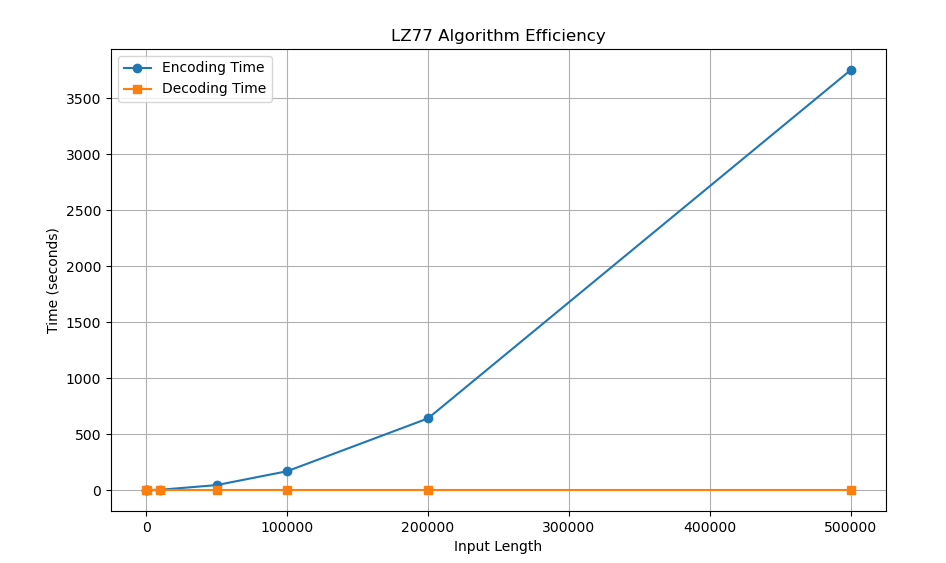
\includegraphics[width=0.8\textwidth]{test.png}
\caption{График зависимости времени выполнения алгоритма LZ77 от длины входных данных}
\label{fig:performance}
\end{figure}

\subsection*{Краткий вывод}

Результаты тестирования показывают, что алгоритм LZ77 подходит для сжатия текста, но требует значительных временных затрат для кодирования при увеличении размера входных данных. В то же время процесс декодирования остаётся крайне эффективным даже для больших объёмов данных.
